\documentclass[utf8]{frontiersSCNS}
\usepackage{url,hyperref,lineno,microtype,subcaption}
\usepackage{color,tensor,multirow,siunitx}
\usepackage[onehalfspacing]{setspace}
\usepackage{makecell}

\renewcommand{\cellalign}{cl}

\newcommand{\ds}{\displaystyle}
\newcommand{\nl}{\ \\ }
\newcommand{\ud}{\textrm{ d}}
\newcommand{\bs}{\bigskip}

\newcommand{\bu}{\mathbf{u}}
\newcommand{\bv}{\mathbf{v}}
\newcommand{\bx}{\mathbf{x}}
\newcommand{\be}{\mathbf{e}}
\newcommand{\bb}{\mathbf{b}}
\newcommand{\bk}{\mathbf{k}}
\newcommand{\bn}{\mathbf{n}}
\newcommand{\bR}{\mathbf{R}}

\definecolor{red}{rgb}{1,0,0}
\definecolor{blue}{rgb}{0,0,0.8}
\definecolor{green}{rgb}{0,0.5,0}
\newcommand{\emphc}[1]{\emph{\textcolor{red}{#1}}}
\newcommand{\replyRone}[1]{\emph{\textcolor{blue}{#1}}}
\newcommand{\replyRtwo}[1]{\emph{\textcolor{green}{#1}}}
\newcommand{\modif}[1]{\textcolor{red}{#1}}
\newcommand{\hycom}{\textsc{hycom} }
\newcommand{\slim}{\textsc{slim}\ }
\newcommand{\ie}{{\it i.e.}\ }
\newcommand{\eg}{{\it e.g.}\ }
\linenumbers

\def\keyFont{\fontsize{8}{11}\helveticabold }
\def\firstAuthorLast{Dobbelaere {et~al.}} %use et al only if is more than 1 author
\def\Authors{Thomas Dobbelaere\,$^{1,*}$, Erinn Muller\,$^{2}$, Lewis Gramer\,$^{3,4}$, Dan Holstein\,$^{5}$  and Emmanuel Hanert\,$^{1,6}$}
\def\Address{
$^{1}$ Earth and Life Institute (ELI), UCLouvain, Louvain-la-Neuve, Belgium \\
$^{2}$ Coral Health and Disease Program, Mote Marine Laboratory, Sarasota, FL, USA \\
$^{3}$ Cooperative Institute for Marine and Atmospheric Studies (CIMAS), University of Miami, Miami, FL, USA \\
$^{4}$ Atlantic Oceanographic and Meteorological Laboratory (AOML), NOAA, Miami, FL, USA \\
$^{5}$ Department of Oceanography and Coastal Sciences, College of the Coast and Environment, Louisiana State University, Baton Rouge, LA, USA \\
$^{6}$ Institute of Mechanics, Materials and Civil Engineering (IMMC), UCLouvain, Louvain-la-Neuve, Belgium \\
}
% The Corresponding Author should be marked with an asterisk
% Provide the exact contact address (this time including street name and city zip code) and email of the corresponding author
\def\corrAuthor{Earth and Life Institute (ELI), UCLouvain, Croix du Sud 2 box L7.05.16, B-1348 Louvain-la-Neuve, Belgium}

\def\corrEmail{thomas.dobbelaere@uclouvain.be}


\begin{document}
\onecolumn
\firstpage{1}

\title[Some alt title]{Some nice title}

\author[\firstAuthorLast ]{\Authors} %This field will be automatically populated
\address{} %This field will be automatically populated
\correspondance{} %This field will be automatically populated
\extraAuth{}

\maketitle
\begin{abstract}
For about five years, the Florida Reef Tract (FRT) has been experiencing an outbreak of the Stony Coral Tissue Loss Disease (SCTLD). First reported off the coast of Miami-Dade County in 2014, the SCTLD outbreak now \emphc{(In April 2020?)} spans from the northern extent of the reef tract in Martin County down to Rock Key in the Lower Keys. However, the causative agent for this outbreak is currently unknown. One hypothesis is that it is transported within composite material (such as coral mucus, dying tissues and/or resuspended sediments) driven by currents and potentially persisting in the water column for extended periods of time. The oceanographic feasibility of this hypothesis has been tested with a three-state (Susceptible, Infected, Removed) epidemiological model spatially driven by connectivity data obtained with the high-resolution ocean model SLIM. SLIM locally achieves a spatial resolution of up to 100 m over the scale of the entire FRT, which allows for the simulation of transport processes at the reef scale. We run this model for the period of May 2018 to March 2019 and investigate three transport modes for the disease causative agents: (i) negatively buoyant particles in the bottom boundary layer; (ii) neutrally buoyant particles in the water column; and (iii) positively buoyant particles in the near-surface layer. Model simulations combining each of these three transport modes with different biological/epidemiological parameters have been investigated in an attempt to reproduce the observed spread of the SCTLD throughout the FRT. Simulations using neutrally buoyant materials as vectors gave the best match with observations. These results strongly suggests that mean barotropic currents drive the propagation of the outbreak.\textcolor{blue}{TODO: update when results/discussion sections done.} \emphc{As it stands, the abstract is too much focused on the methodology and not enough on the results and their implication...} 

\tiny
\keyFont{ \section{Keywords:} Some nice keywords} 
\end{abstract}

% === INTRODUCTION === %
\section{Introduction}
Stony Coral Tissue Loss disease: where, when, what do we know (tank based transmission exp, spatial modeling paper)
SIR modeling background?
Hydrodynamic modeling?
The objective...

% === METHODS === %
\section{Methods}

% --> Subsection 1
\subsection{Modeling the exchanges of infectious material between reefs}
The exchanges of infectious material between coral reefs are primarily driven by ocean currents, which therefore have to be accurately simulated. An ocean model should provide a realistic large-scale circulation while also resolving small-scale flow features down to the scale of individual reefs. In this study, we use the unstructured-mesh depth-integrated coastal ocean model SLIM\footnote{{\tt https://www.slim-ocean.be}} to simulate ocean currents over an area that includes the FRT but also the Florida Strait and part of the Gulf of Mexico (Fig. \ref{fig:setup}). By using an unstructured mesh, we can increase the model resolution only over the FRT and hence concentrate computational resources where they are most needed. SLIM, being a depth-averaged model, is well suited to shallow-water flows. On the shelf break and in deeper areas, it might however not be able to model more complex processes such as mesoscale eddies that are observed along the southern flank of the FRT and the thermally-driven FC. This issue has been partly circumvented by relaxing SLIM's velocity towards the depth-averaged velocity obtained with the HYbrid Coordinate Ocean Model (HYCOM, \cite{Chassignet2007}) implemented over the Gulf of Mexico, when the water depth exceeds a certain threshold. Details of the model formulation and validation are provided in \cite{frys20}. 

\begin{figure}
    \centering
    \includegraphics[width=.8\textwidth]{figures/setup_2.png}
    \caption{Top row: Model computational domain with the bathymetry (left), and the unstructured mesh (right). The mesh contains about $7 \times 10^5$ elements and the resolution varies between about 100 m and 2.5 km. Close-up views of the mesh (middle) and snapshots of the currents on May, 25 2018 at 00:00 (bottom), for the Marquesas Keys (left) and the Lower Keys (right). This illustrates the benefits of unstructured meshes to represent the fine-scale details of the topography and hence simulate currents down to the scale of individual reefs (shown in light grey) and islands (shown in black). \emphc{EH: You will have to update this figure as it is too close from the one in our FRT connex paper.}}
    \label{fig:setup}
\end{figure}

The mesh resolution depends only on the distance to the coast but we distinguish between the coastlines along the FRT where we impose a maximum resolution of 100 m and the other coastlines along which the maximum resolution is 2500 m. The mesh has been generated with the open-source mesh generator GMSH \citep{Geuzaine2009} and is shown in Fig. \ref{fig:setup}. It has about $7 \times 10^5$ elements. The coarsest elements, far away from the FRT, have a size of about 10 km. An illustration of ocean currents simulated on that mesh are shown in Fig. \ref{fig:setup}. It shows how a 100-m spatial resolution allows us to simulate fine-scale details of the flow, such as recirculation eddies and currents within the dense reef system in the Lower Keys that consist of many individual reefs with narrow passages in between. 

The simulated currents can then be used to model dispersal of infectious material throughout the FRT. In this study, 3 types of potential vector for the disease causative agent were considered: positively buoyant (e.g. mucus and surfactant), neutrally buoyant (e.g. fines, pelagic organisms) and negatively buoyant (e.g. sediments, composites, demersal organisms). As SLIM is a depth-averaged model, the mean currents its generate are well suited to model the dispersal of neutrally buoyant material remaining within the water column. However, these currents must be modified to correctly represent the dynamics of materials evolving in the surface and bottom boundary layers. Therefore, the impact of surface stokes drift on positively buoyant materials is estimated by adding 1.5\% of the wind speed to SLIM currents with a windage angle of 45$^\circ$ to the right, as described in \citep{ardhuin2009observation} \emphc{(I think this needs to be further developed as it is quite important... Discuss effect of waves and Stokes drift}. For negatively buoyant materials, on the other hand, bottom currents are obtained by taking 60\% of SLIM currents velocity with a veering angle of 15$^\circ$ to the left \emphc{(explain why)}\textcolor{blue}{TD: Ekman ? Check with Lew...}.

Using these three velocity fields, the next step is to release virtual particles on all the reefs composing the FRT to model the dispersal of infected materials carrying the disease causative agent. To do so, a map of the location of the different reefs of Florida has been used. We use the layer giving the areas where coral reefs and hardbottom are found from the Unified Florida Reef Tract Map \citep{fwc2017unified} that we then further divide into 500 m squares, generating a total of 16823 polygons \textcolor{red}{(14058 without the big Vaca reef)}. At the beginning of each simulated months and for each type of currents, a total of about $1.5 \times 10^6$ particles are released over all the reef polygons. These particles have a state composed of their polygon of origin as well as their mass, initialized to 1, that they loose at a constant rate $\gamma$ as they are displaced by surface, mean or bottom currents. \textcolor{blue}{As monthly simulations are performed, the value of $\gamma$ is chosen so that particles have a half life of 30 days}. When the particles are brought over reef polygons by currents, the amount of infected mass that lands on the polygon is recorded in monthly potential connectivity matrices whose entries are denoted $C_{ij}$. The matrix rows correspond to the source reefs and the columns correspond to the destination reefs. Hence $C_{ij}$ represents the mass of of infected material originating from sub-reef i that have settled on sub-reef j. This matrix can then be normalized by dividing each of its rows $i$ by the the total mass of particles released on polygon $i$ in order to obtained the normalized potential connectivity matrix $\tilde{C}$, whose entry $\tilde{C}_{ij}$ gives the probability that infectious material produced on sub-reef $i$ settles on sub-reef $j$

% --> Subsection 2
\subsection{Epidemiological modeling}
% --> Subsubsection 2.1
\subsubsection{Model equations}
The spread of the SCTLD throughout the FRT is simulated using a connectivity-based Kermack-McKendrick SIR model. SIR models are among the most standard epidemiological models. They divide individuals into three compartments: susceptible (S), infectious (I) and removed (R). When affected by the disease, susceptible individuals become infectious and infect other susceptible individuals until they are removed, either by recovery or death. Such models usually rely on the hypothesis of an homogeneous, well-mixed population. To account for the spatial heterogeneity of the FRT, the basic SIR formulation is here modified by considering the proportions of susceptible ($S_j$), infectious ($I_j$) and removed ($R_j$) corals of each polygon reef $j$. In this epidemiological model, individual reefs interact through the exchange of infectious material as represented by the connectivity matrix. For each sub-reef $j$ and at any time, the following relations hold: $0\leq S_j,I_j,R_j\leq 1$ and $S_j+I_j+R_j=1$. The evolution of these proportions through time is governed by the following equations:
% * <Daniel Holstein> 08:42:59 30 Apr 2020 UTC-0500:
% There is also some novelty to this approach.
% * <Daniel Holstein> 08:41:59 30 Apr 2020 UTC-0500:
% Agreed. I can provide some background and coral disease references here.
% ^ <thomas.dobbelaere@uclouvain.be> 16:24:09 04 May 2020 UTC+0200:
% That would be nice. Thank you
\begin{equation}
    \begin{aligned}
        \dfrac{dS_j}{dt} &= -\beta\sum_i\dfrac{A_i}{A_j}I_i\tilde{C}_{ij}S_j - \beta'(I_j)S_jI_j \\
        \dfrac{dI_j}{dt} &= \beta\sum_i\dfrac{A_i}{A_j}I_i\tilde{C}_{ij}S_j + \beta'(I_j)S_jI_j - \sigma I_j \\
        \dfrac{dR_j}{dt} &= \sigma I_j
    \end{aligned}\label{eq:epidemio}
\end{equation}
where $\tilde{C}_{ij}$ is the entry of reef $(i,j)$ of the normalized potential connectivity matrix [-], $A_i$ is the area of reef polygon $i$ [km$^2$], $\sigma$ is the removal rate [s$^{-1}$], and $\beta$ and $\beta'(I_j)$ are the inter- and intra-reef disease transmission rates [s$^{-1}$], respectively. In this model, infectious corals of reef $i$ can infect corals of reef $j$ if there is non-zero probability of infectious material exchange from reef $i$ to reef $j$, given by $\tilde{C}_{ij}$. Moreover, to account for coral resistance to the disease, the intra-reef transmission function $\beta'(I_j)$ has the shape of a smooth step function of the proportion of infectious corals $I_j$ and writes:
\begin{equation}
    \beta'(I_j) = \dfrac{\beta_0'}{2}(1+\tanh[(I_j-I_0)/\tau]),\label{eq:beta}
\end{equation}
where $I_0$ is a threshold on the infection population above which intra-reef transmission becomes significant, and $\tau$ is a measure of the interval over which the transition for low to high transmission occurs. As long as the proportion of infectious corals on reef $j$ is below $I_0$, the only infection mechanism taking place is connectivity-driven transmission at rate $\beta$. Once the threshold is exceeded ( $I_j \geq I_0$ ), intra-reef transmission with rate $\beta'_0$ is activated. A larger value of threshold $I_0$ corresponds to a greater resistance to disease for corals and therefore a slower spread of the disease within reef $j$. For this study the same values were used for $\beta$ and $\beta'_0$.

\subsubsection{Calibration of the model coefficients}
Values of $\sigma$ and $\beta_0'$ are fitted to observations in order to accurately simulate the temporal evolution of $S_j,I_j,R_j$ on each infected reef polygon. To do so, Eqs $\ref{eq:epidemio}$, representing the disease dynamics through the entire FRT, are simplified to a single-reef SIR system:
% * <emuller@mote.org> 06:44:25 05 May 2020 UTC-0400:
% Do we want to include the parameter estimations from the meta-analysis to show that they are reasonable and valid, or would this go in the discussion?
\begin{equation}
    \begin{aligned}
        \dfrac{dS}{dt} &= -\beta'_0SI \\
        \dfrac{dI}{dt} &= \beta'_0SI - \sigma I \\
        \dfrac{dR}{dt} &= \sigma I
    \end{aligned}\label{eq:simplified}
\end{equation}
Eqs \ref{eq:simplified} give a reasonable approximation of the evolution of the disease on sub-reefs for which $I_j > I_0$, as intra-reef infection, when activated, is the dominant infection mechanism. Using this approximation, the ratio $\beta_0'/\sigma$ is found by imposing that the proportion of susceptible corals that remains after the disease has vanished ($S_\infty$) matches with the observations. A standard property of a SIR model solution is that
\begin{equation}
    S_\infty - \frac{\sigma}{\beta_0'}\log(S_{\infty}/S_0) = 1\label{eq:ratio}
\end{equation}
where the initial proportion of susceptible corals is taken equal to $1-I_0$ (see for instance \cite{Murray07}). The ratio $\beta'_0/\sigma$ is then used to find the value of $\beta'_0$ that reproduces the observed temporal evolution of the state of the coral colonies, as shown in figure \ref{fig:calibration}. The calibrated values of the transmission and removal rates are then given by $\beta_0'=6.45$ days$^{-1}$ and $\sigma=7$ days$^{-1}$. This derived characteristic transmission time agrees with direct measurements in tanks as the average transmission time observed during experiments was about 10.5 days.
% * <emmanuel.hanert@uclouvain.be> 21:10:47 06 May 2020 UTC+0200:
% OK, but you don't say how do you find the value of sigma...
% ^ <thomas.dobbelaere@uclouvain.be> 09:13:12 07 May 2020 UTC+0200:
% The value of sigma is obtained using the beta/sigma ratio

\begin{figure}
    \centering
    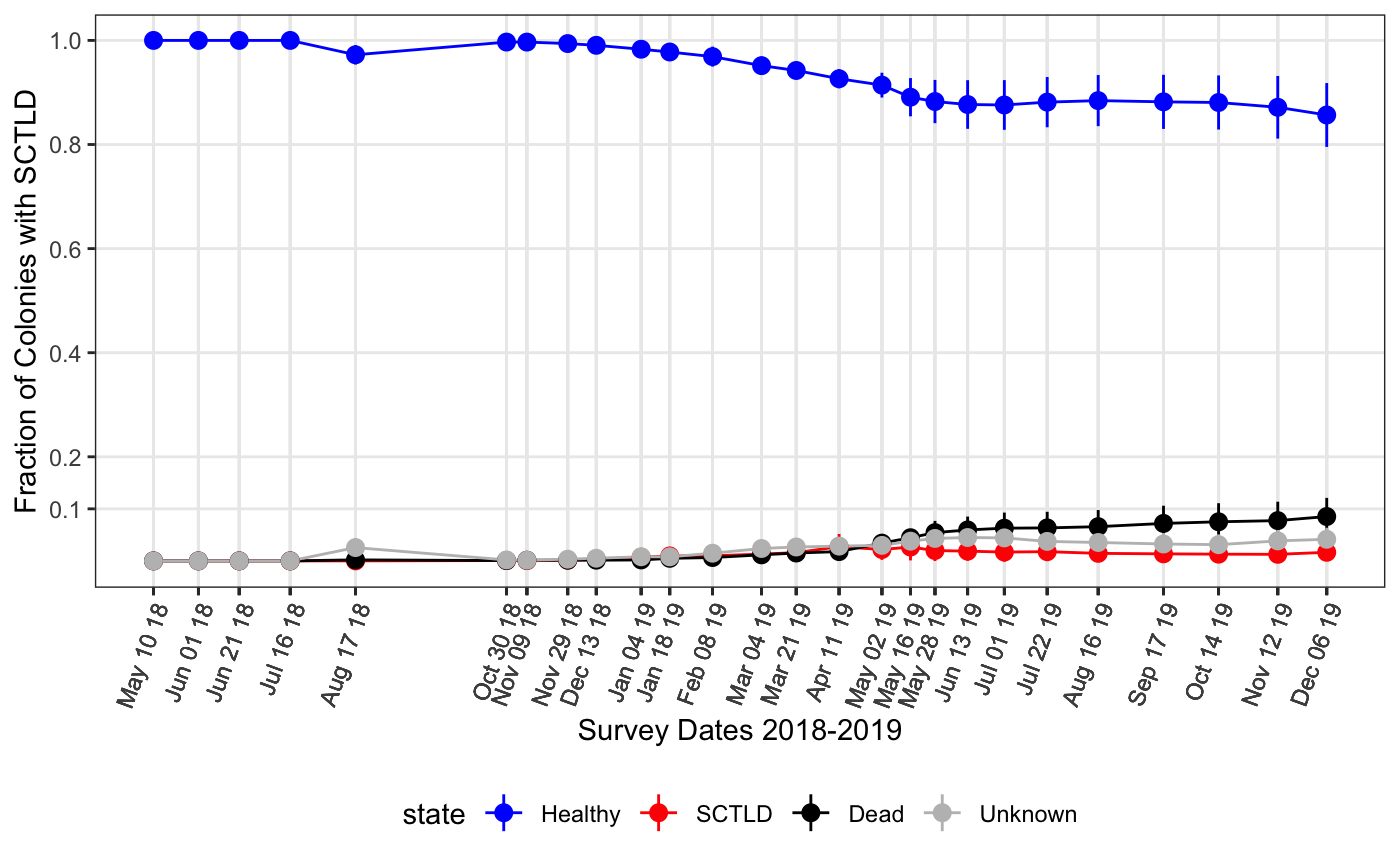
\includegraphics[width=.7\textwidth]{figures/image2.png}
    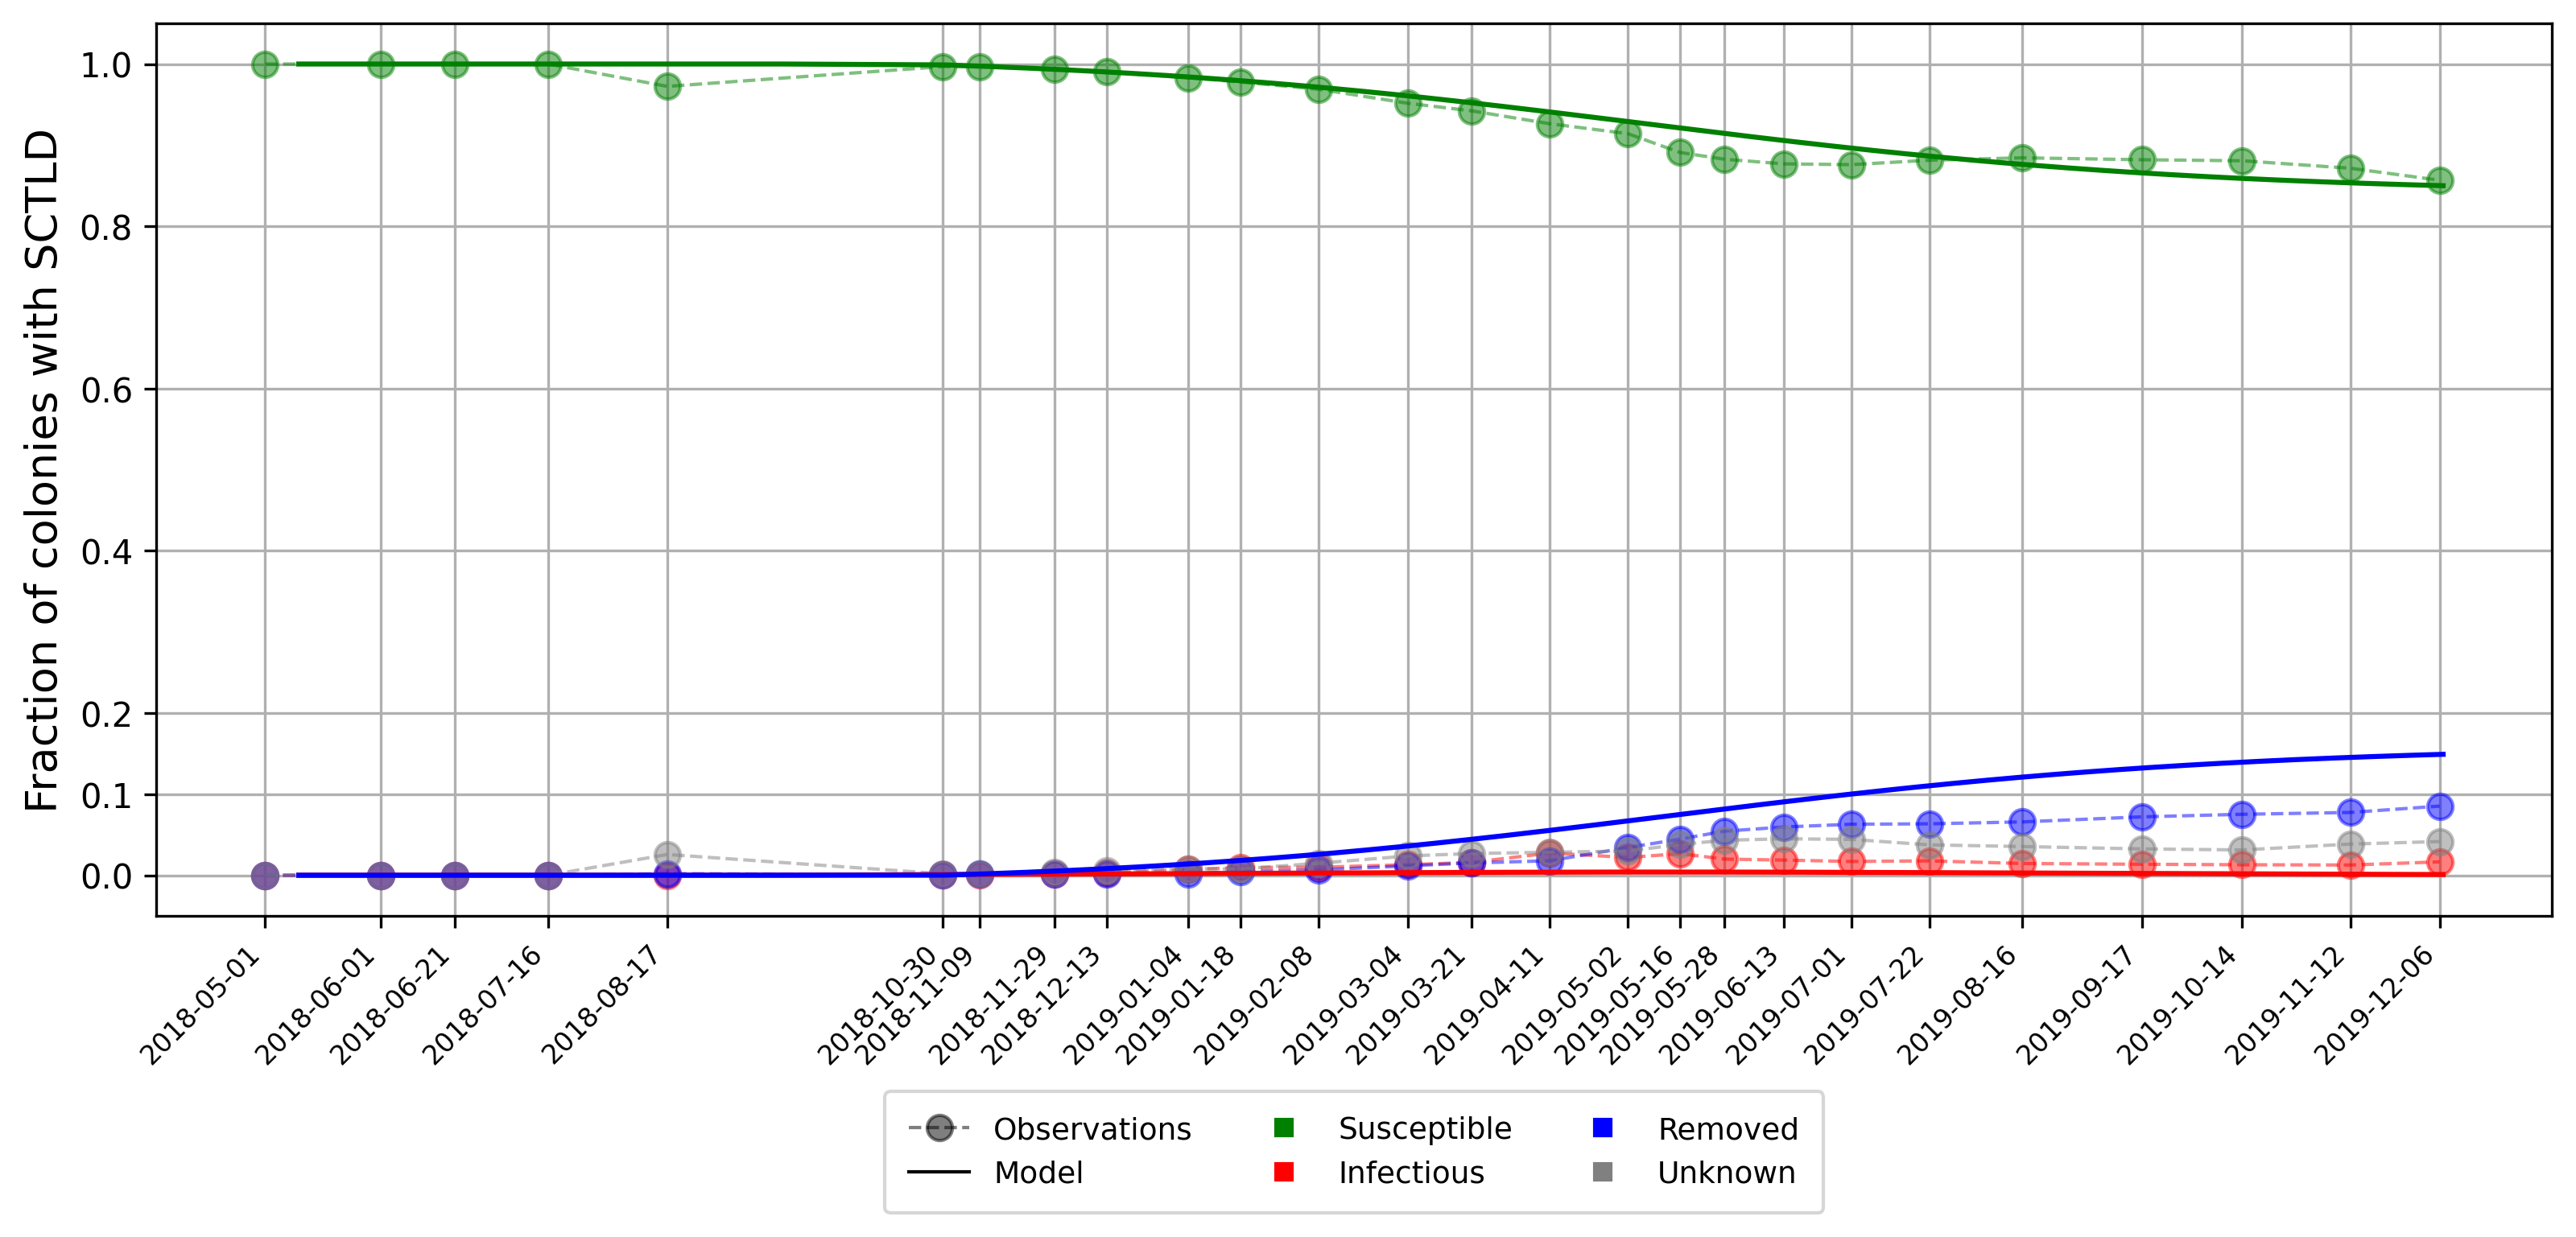
\includegraphics[width=.69\textwidth]{figures/sir_obs.png}
    \caption{\textbf{Above:} Observed disease prevalence over time (all colonies from all sites), error bars are the 95\% confidence intervals. \textbf{Below:} Modeled disease prevalence over time usi ng equations \ref{eq:simplified} using calibrated transmission and removal parameters  $\beta_0'=6.45$ days$^{-1}$ and $\sigma=7$ days$^{-1}$. \emphc{This figure could probably be improved by showing observations and models results on the same graph...} \textcolor{blue}{To do: ask data to Erinn}}
    \label{fig:calibration}
\end{figure}
\subsubsection{Initialization of the model}
In order to solve Eqs. \ref{eq:epidemio}, initial conditions are needed, \ie proportions of susceptible, infectious and recovered corals at the beginning of the simulated period. This information is constructed based on different field-collected datasets: : (i) Coral Reef Evaluation and Monitoring Project (CREMP; 2014–2017), (ii) CREMP Presence/Absence Data (CREMP P\_A; 2016–2017), (iii) Southeast Florida Coral Reef Evaluation and Monitoring Project (SECREMP; 2014– 2017), (iv) Florida Reef Resilience Program Disturbance Response Monitoring (FRRP; 2014–2017), (v) Hurricane Irma Rapid Reef Assessment (IRMA; 2017, \cite{viehman2018}), (vi) the Southeast Florida Action Network citizen science program (SEAFAN; 2014–2017), and (vii) the Southern Coral Disease Margin field effort (2017; \cite{neely2018surveying}). These datasets give the locations and dates at which the SCTLD has been observed throughout the FRT. Using this information, we first delineate an infected zone by constructing the concave hull of the points where the disease was observed before May 2018. The reefs infected prior to the beginning of our simulated period are then defined as the reefs located inside the constructed zone. The time of observed infection is then spatially interpolated on each reef of the infected zone by kriging with a Gaussian semivariogram using Python \texttt{pyKrige} module. Assuming a state $(S,I,R)=(1-I_0, I_0, 0)$ when the disease was observed, the proportions of susceptible, infectious and removed corals on each reef of the infected zone on the 1st May 2018 is finally approximated using the simplified equations \ref{eq:simplified}. Reefs outside of the infected zone are initialized with a population of 100\% of susceptible corals.  
\subsubsection{Disease front displacement rate computation}
\begin{figure}
    \centering
    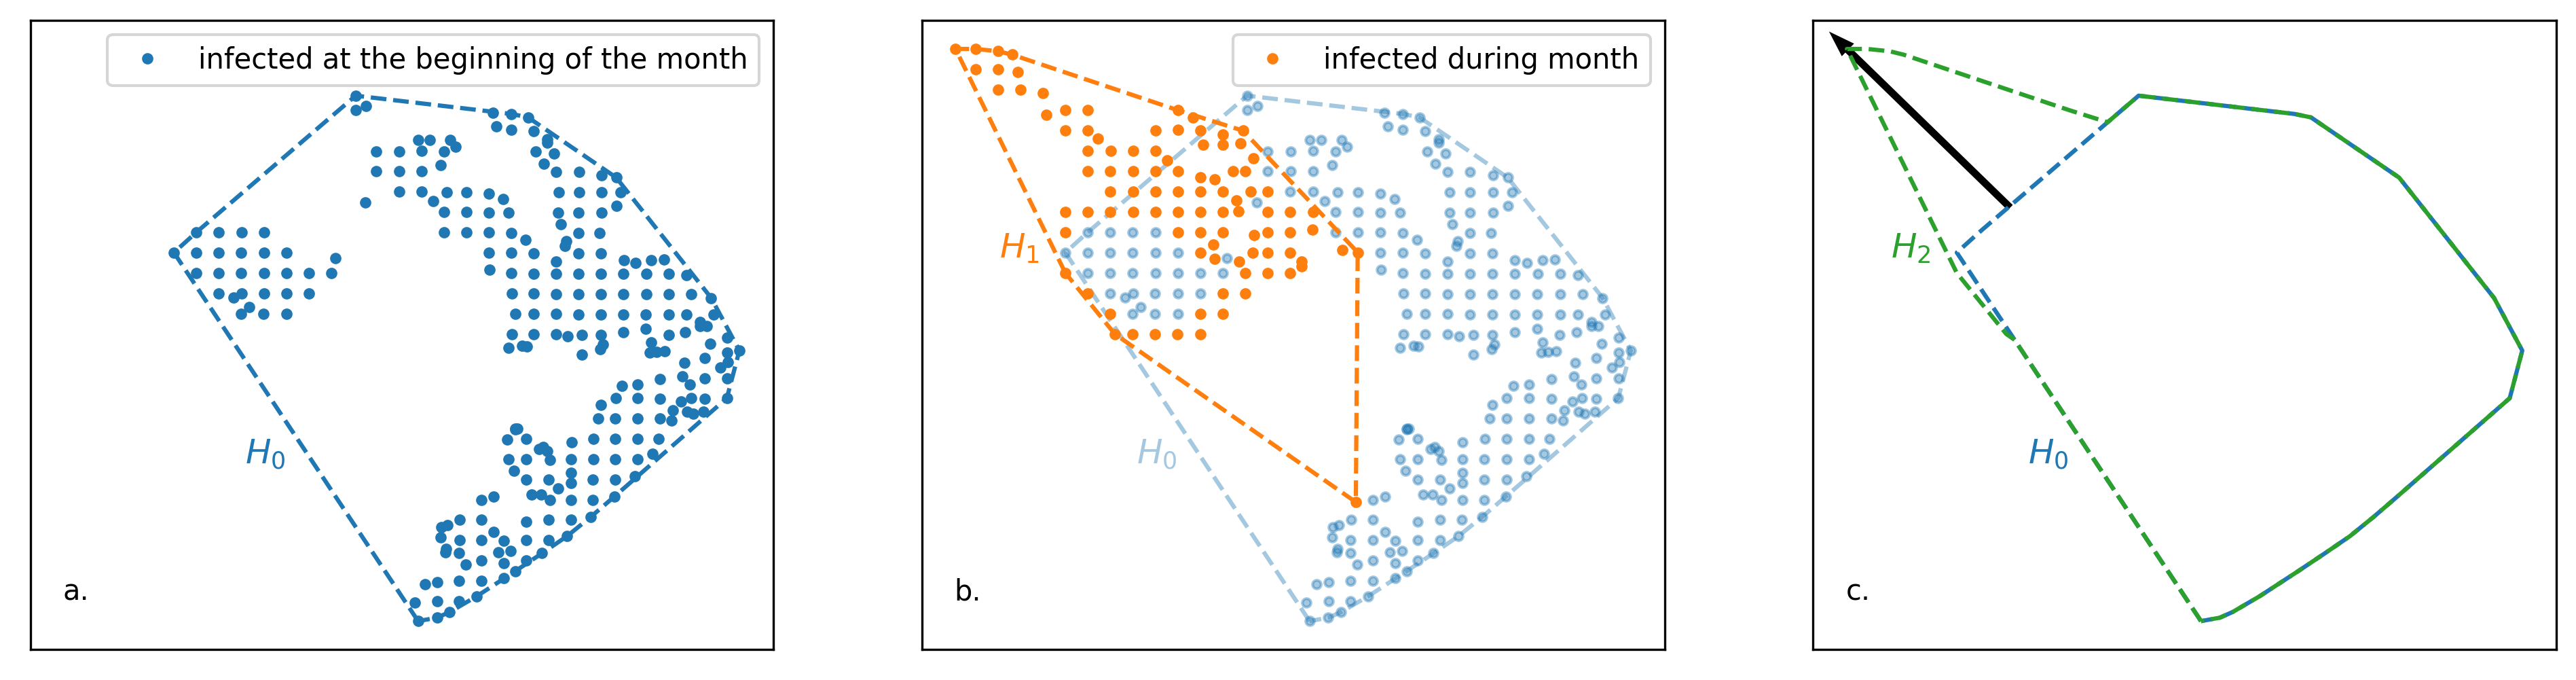
\includegraphics[width=.95\textwidth]{figures/hull_example.png}
    \caption{Method used to compute the disease front displacement during each simulated month.\textbf{a.} Concave hull of the infected polygons at the beginning of the simulated month $H_0$. \textbf{b.} Concave hull of the polygons infected during the simulated month $H_1$. \textbf{c.} Arrow showing the computed front displacement during simulated month between $H_0$ and $H_2$, the union of $H_0$ and $H_1$.}
    \label{fig:hull}
\end{figure}
\citep{muller2020spatial} estimated the speed of the spreading STCLD epidemics at around 92 m/day in the southern section of the FRT. In order assess our simulation results in regard to this value, we developed a methodology to compute the displacement of the disease front during each modeled month show. First, the concave hull of the infected polygons at the beginning of the simulated month $H_0$ is computed. Then the concave hull of the polygons infected during the simulated month $H_1$ is computed while the concave hull $H_2$ is defined as the union of $H_0$ and $H_1$. This methodology is illustrated in figure \ref{fig:hull}. The distance traveled by the disease front is then obtained by computing:
\begin{equation}
    \max\limits_{\mathbf{x}_2\in H_2}\min\limits_{\mathbf{x}_0\in H_0} \|\mathbf{x}_2 - \mathbf{x}_0\|_2
\end{equation}
The epidemics front speed is finally computed by dividing the resulting distance by the number of days in the simulated month. As the front speed of \citep{muller2020spatial} is derived from quarterly- or annually-identified disease front, the average of our monthly speeds is used for comparison with the 92 m/day reference value.

% === RESULTS === %
\section{Results}

\subsection{Exchanges of infected materials}
Connectivity matrices are obtained for mean, bottom and surface currents for all simulated months. These matrices can be more easily handled by interpreting them as large graphs whose vertices are reefs. Such networks can then be analyzed using graph theory tools such as the weighted connectivity length (WCL), \ie the average dispersal distance from origin to destination for material produced on a given reef. The weighted connectivity of reef polygon $j$ writes:
\begin{equation}
    WCL_j = \dfrac{\sum_i \tilde{C}_{ji} L_{ji}}{\sum_i \tilde{C}_{ji}}
\end{equation}
where $L_{ji}$ is the distance between reef polygons $j$ and $i$. In addition to this metric, indicators such as the probability of exchange between reefs as well as the number of outgoing connections per reef can be computed. The mean values of these indicators for each type of currents are given in table \ref{tab:connect}. Bottom currents give the networks with smallest WCL and outdegree, suggesting that they drive infected materials on shorter geographical ranges and fewer reefs that the other two types of currents. However, as bottom currents also exhibit the largest average connection probability, they tend to exchange more infectious matter between connected reefs. Mean and surface currents, on the other hand, generate networks with similar WCL. However, although both currents show analogous spreading ranges, exchanges are almost twice smaller with surface currents and occur between less reefs.  This is imputable to the effect of the winds that prevent infectious materials to durably settle on reefs (see Discussion)

\begin{table}
    \centering
    \begin{tabular}{|l|c|c|c|}
        \hline
                                   & mean currents      & bottom currents    & surface currents   \\
        \hline
        \makecell{mean weighted \\
        connectivity length [km]}  & 20.63              & 12.25              & 21.39              \\
        \hline
        \makecell{mean exchange 
        \\probability}             & $2.9\cdot 10^{-4}$ & $7.5\cdot 10^{-4}$ & $1.8\cdot 10^{-4}$ \\
        \hline
        \makecell{mean outgoing \\
        degree}                    & 416                & 159                & 321 \\
        \hline
    \end{tabular}
    \caption{Mean values of the graph theory indicators used to analyze the connectivity matrices obtained with mean, bottom and surface currents}
    \label{tab:connect}
\end{table}

\subsection{Epidemiological model results}
A summary of the epidemiological model results for each type of currents and different values of the infection threshold $I_0$ are shown in figure \ref{fig:results}. Two metrics are used to assess the accuracy of the model. First, the modeled front speed is compared to the reference rate of 92 m/day derived by \citep{muller2020spatial}. Furthermore, we compute the mean of the distances between each point where the SCTLD has been observed during our simulated period and the centroid of the closest reef polygon predicted to be infected by our model during the same period. Figure \ref{fig:results} show that mean barotropic currents perform the best regarding both criteria with a front speed of ~120 m/day and a mean accuracy of ~2 km; while surface currents produce the worst results with respect to both front speed and proximity to the observed affected reefs. Moreover, an interval of optimal values of the infection threshold $I_0$ is observed for both mean and bottom currents between $I_0=5 \times 10^{-4}$ and $I_0=10^{-3}$. For $I_0 > 10^{-3}$, intra-reef infection is strongly impeded and populations of infectious individuals on infected reefs are not sufficiently large to infect other colonies on reefs they are connected to. For values of $I_0$ lower than $5 \times 10^{-4}$ on the other hand, intra-reef infection dominates and coral population on infected reefs is removed too fast to efficiently spread the disease through the network.

\begin{figure}
    \centering
    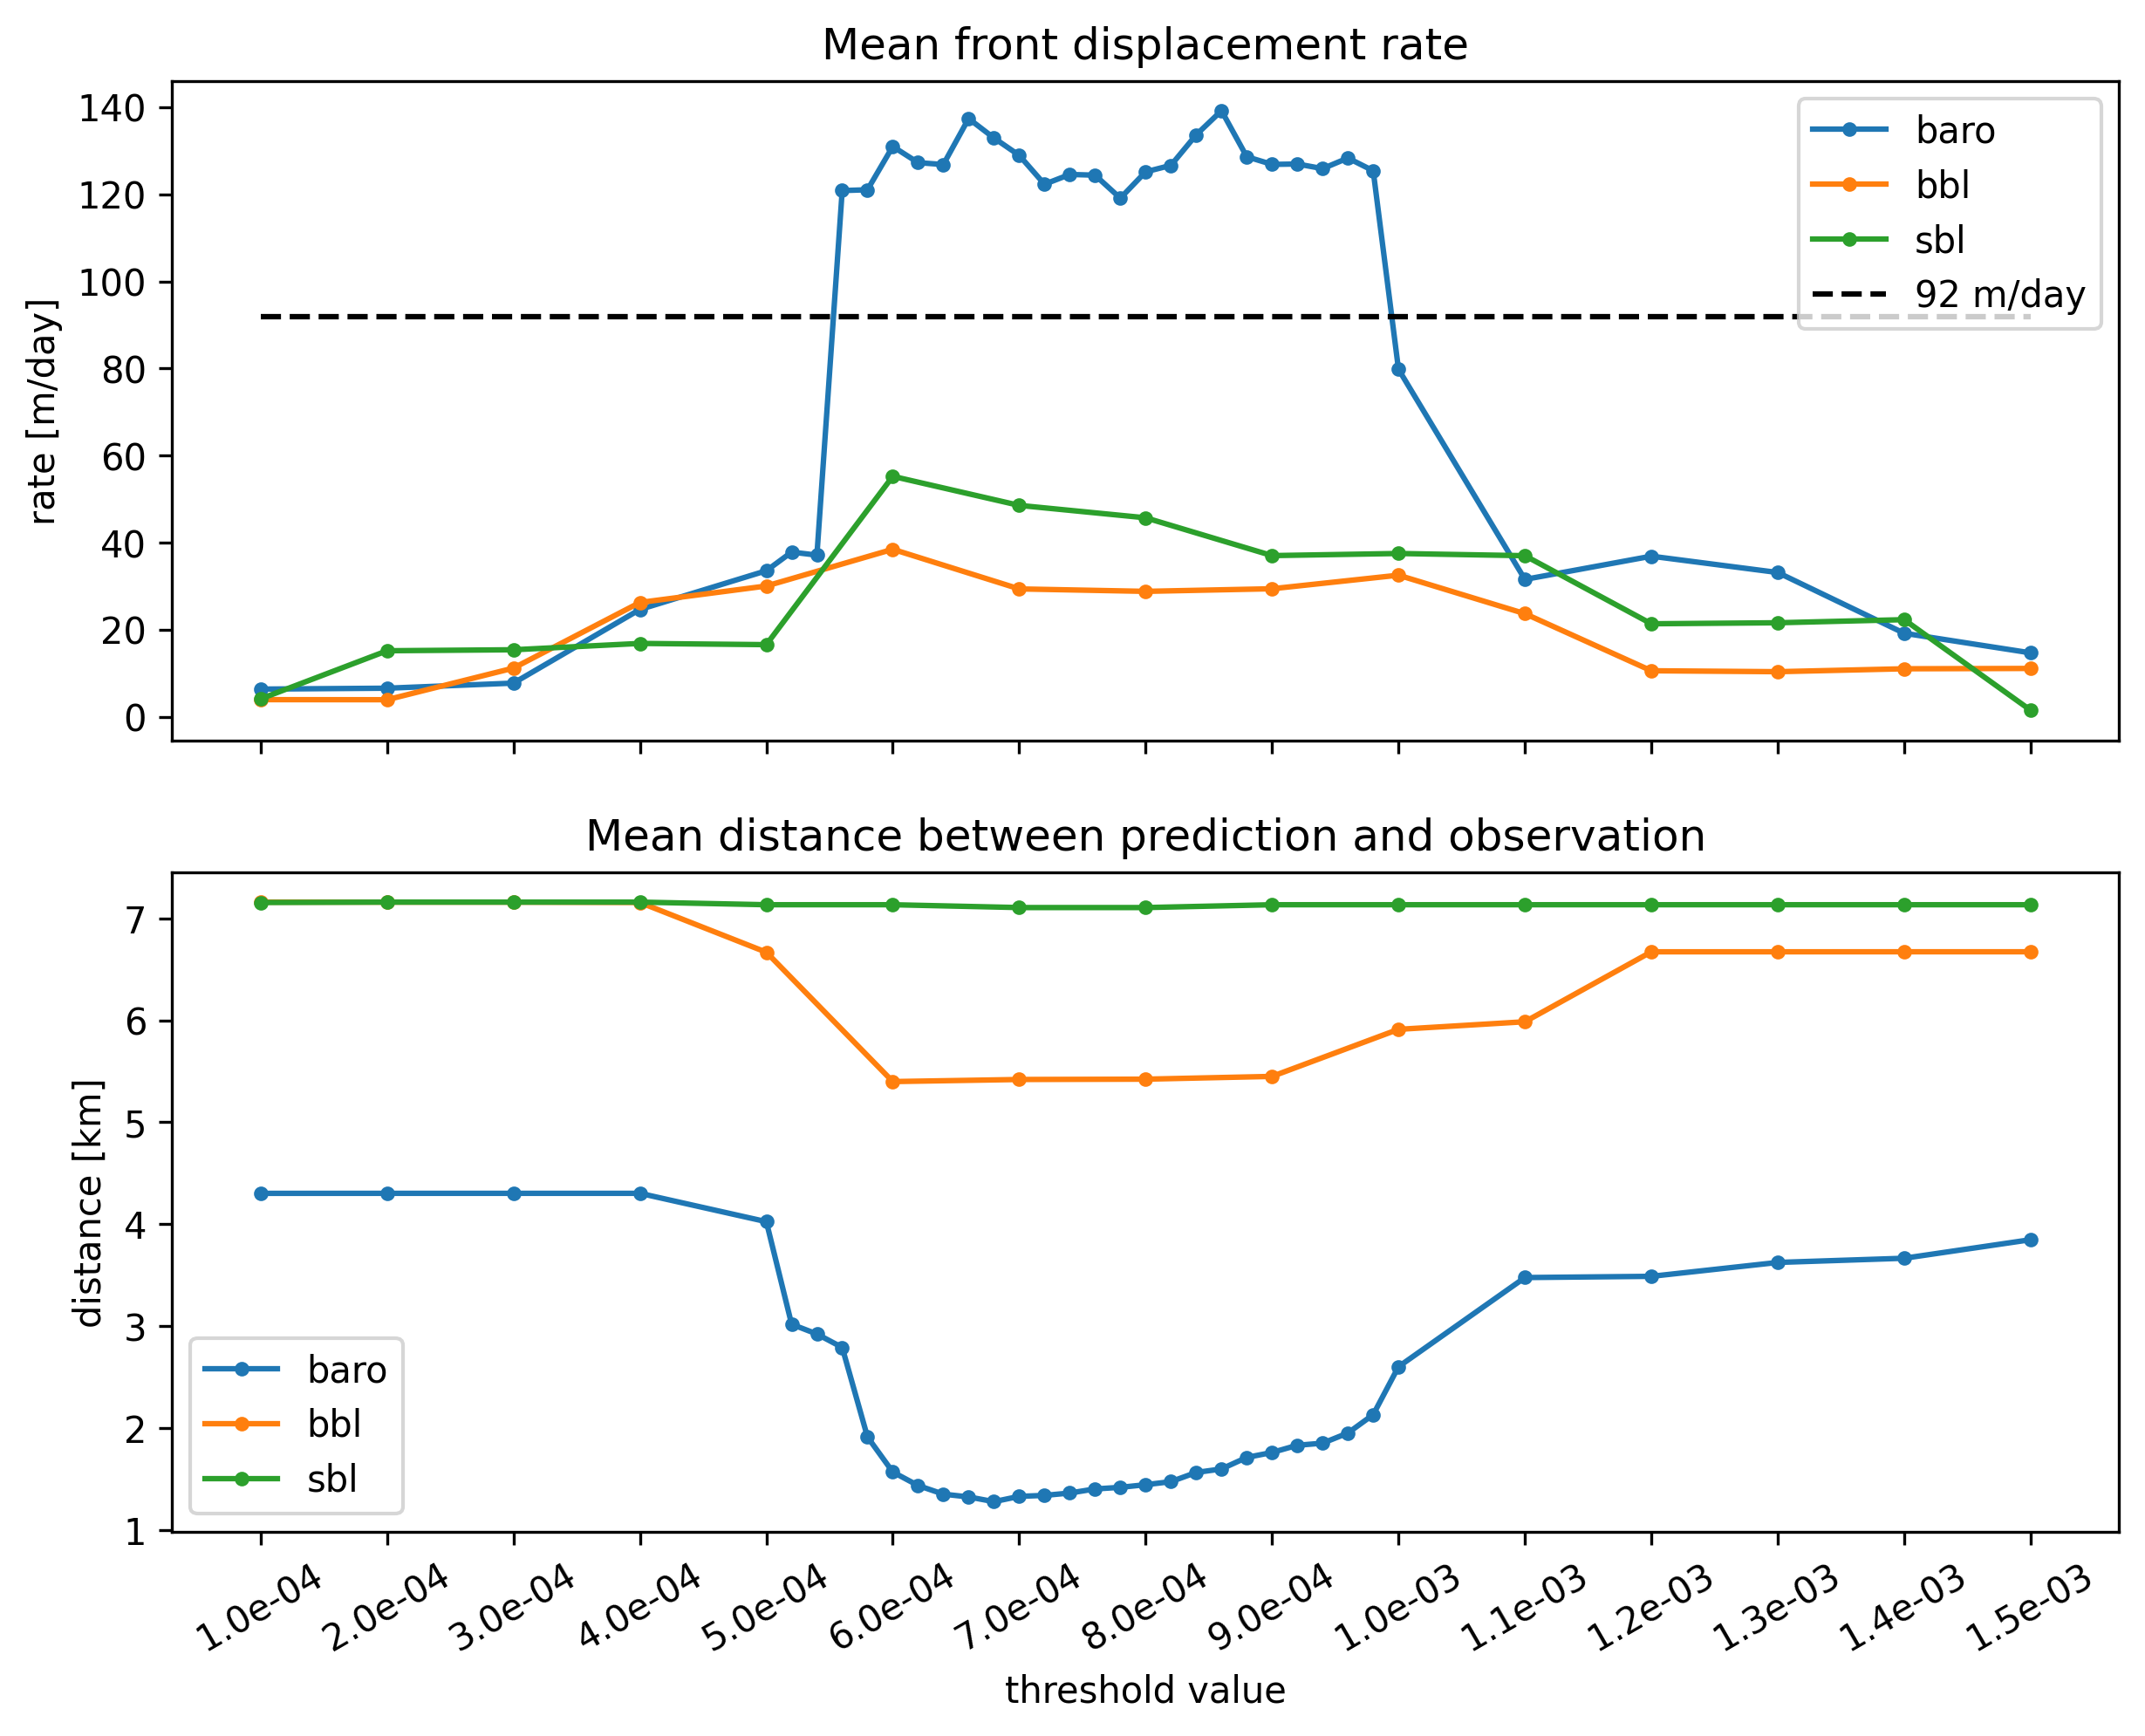
\includegraphics[width=.8\textwidth]{figures/sctld_validation_alt_v3.png}
    \caption{Take home messages:
    \begin{itemize}
        \item Mean currents closest to field data
        \item Good match with observation (predictions is 3km from observations on average) 
    \end{itemize}}
    \label{fig:results}
\end{figure}

The differences between the three modeled types of currents shown in figure \ref{fig:results} can be explained by analyzing the trajectories of the particles used to model the transport of the vector of the causative agent of the disease, as illustrated in Fig. \ref{fig:traj}. Due to the impact of wind on positively buoyant materials, particles driven by surface currents are likely to be blown away from the reefs (see upper part of Fig. \ref{fig:traj}). Moreover, even when winds are pushing particles along the reef line, these particles spend less time over the same region than particles driven by mean and bottom currents (see lower part of Fig. \ref{fig:traj}. Smaller amounts of particle mass will therefore settle on reef polygons, leading to lower entries of the potential connectivity matrix, \ie lower exchange probabilities between reefs. Hence, despite being able to displace infected materials on greater distances, surface currents are less likely to drive the propagation of the disease. Particles driven by bottom currents, on the other hand, remain longer over the same region, producing larger entries of the potential connectivity matrix. Due to these large exchange probabilities between reefs, bottom currents are better at propagating the disease (Fig. \ref{fig:results}). Nevertheless, bottom currents being relatively slower, exchanges of infected materials occur on a limited geographical range. Mean barotropic currents, that carry particles on greater distances while allowing for sufficiently large amounts of infected mass to settle on reef polygons, are thus best suited to propagate the disease (Fig. \ref{fig:results}).

The results shown in figure \ref{fig:results} were obtained by removing the large reef located North to Vaca key, denoted Vaca reef as in \citep{frys20} from our reef polygons. Our first simulations showed that this reef has close to no impact on the modeled spread of the disease to the rest of the FRT. However, as coral coverage is not taken into account in this model, the simulated propagation of the SCTLD on this reef generates unrealistically strong front speed variations due to its large size. As result of the low coral coverage of Vaca reef ($0-10\%$) and the absence of SCTLD observations on this reef, it has therefore been removed from the reef map in order to avoid to overestimate the propagation of the front.

\begin{figure}
    \centering
    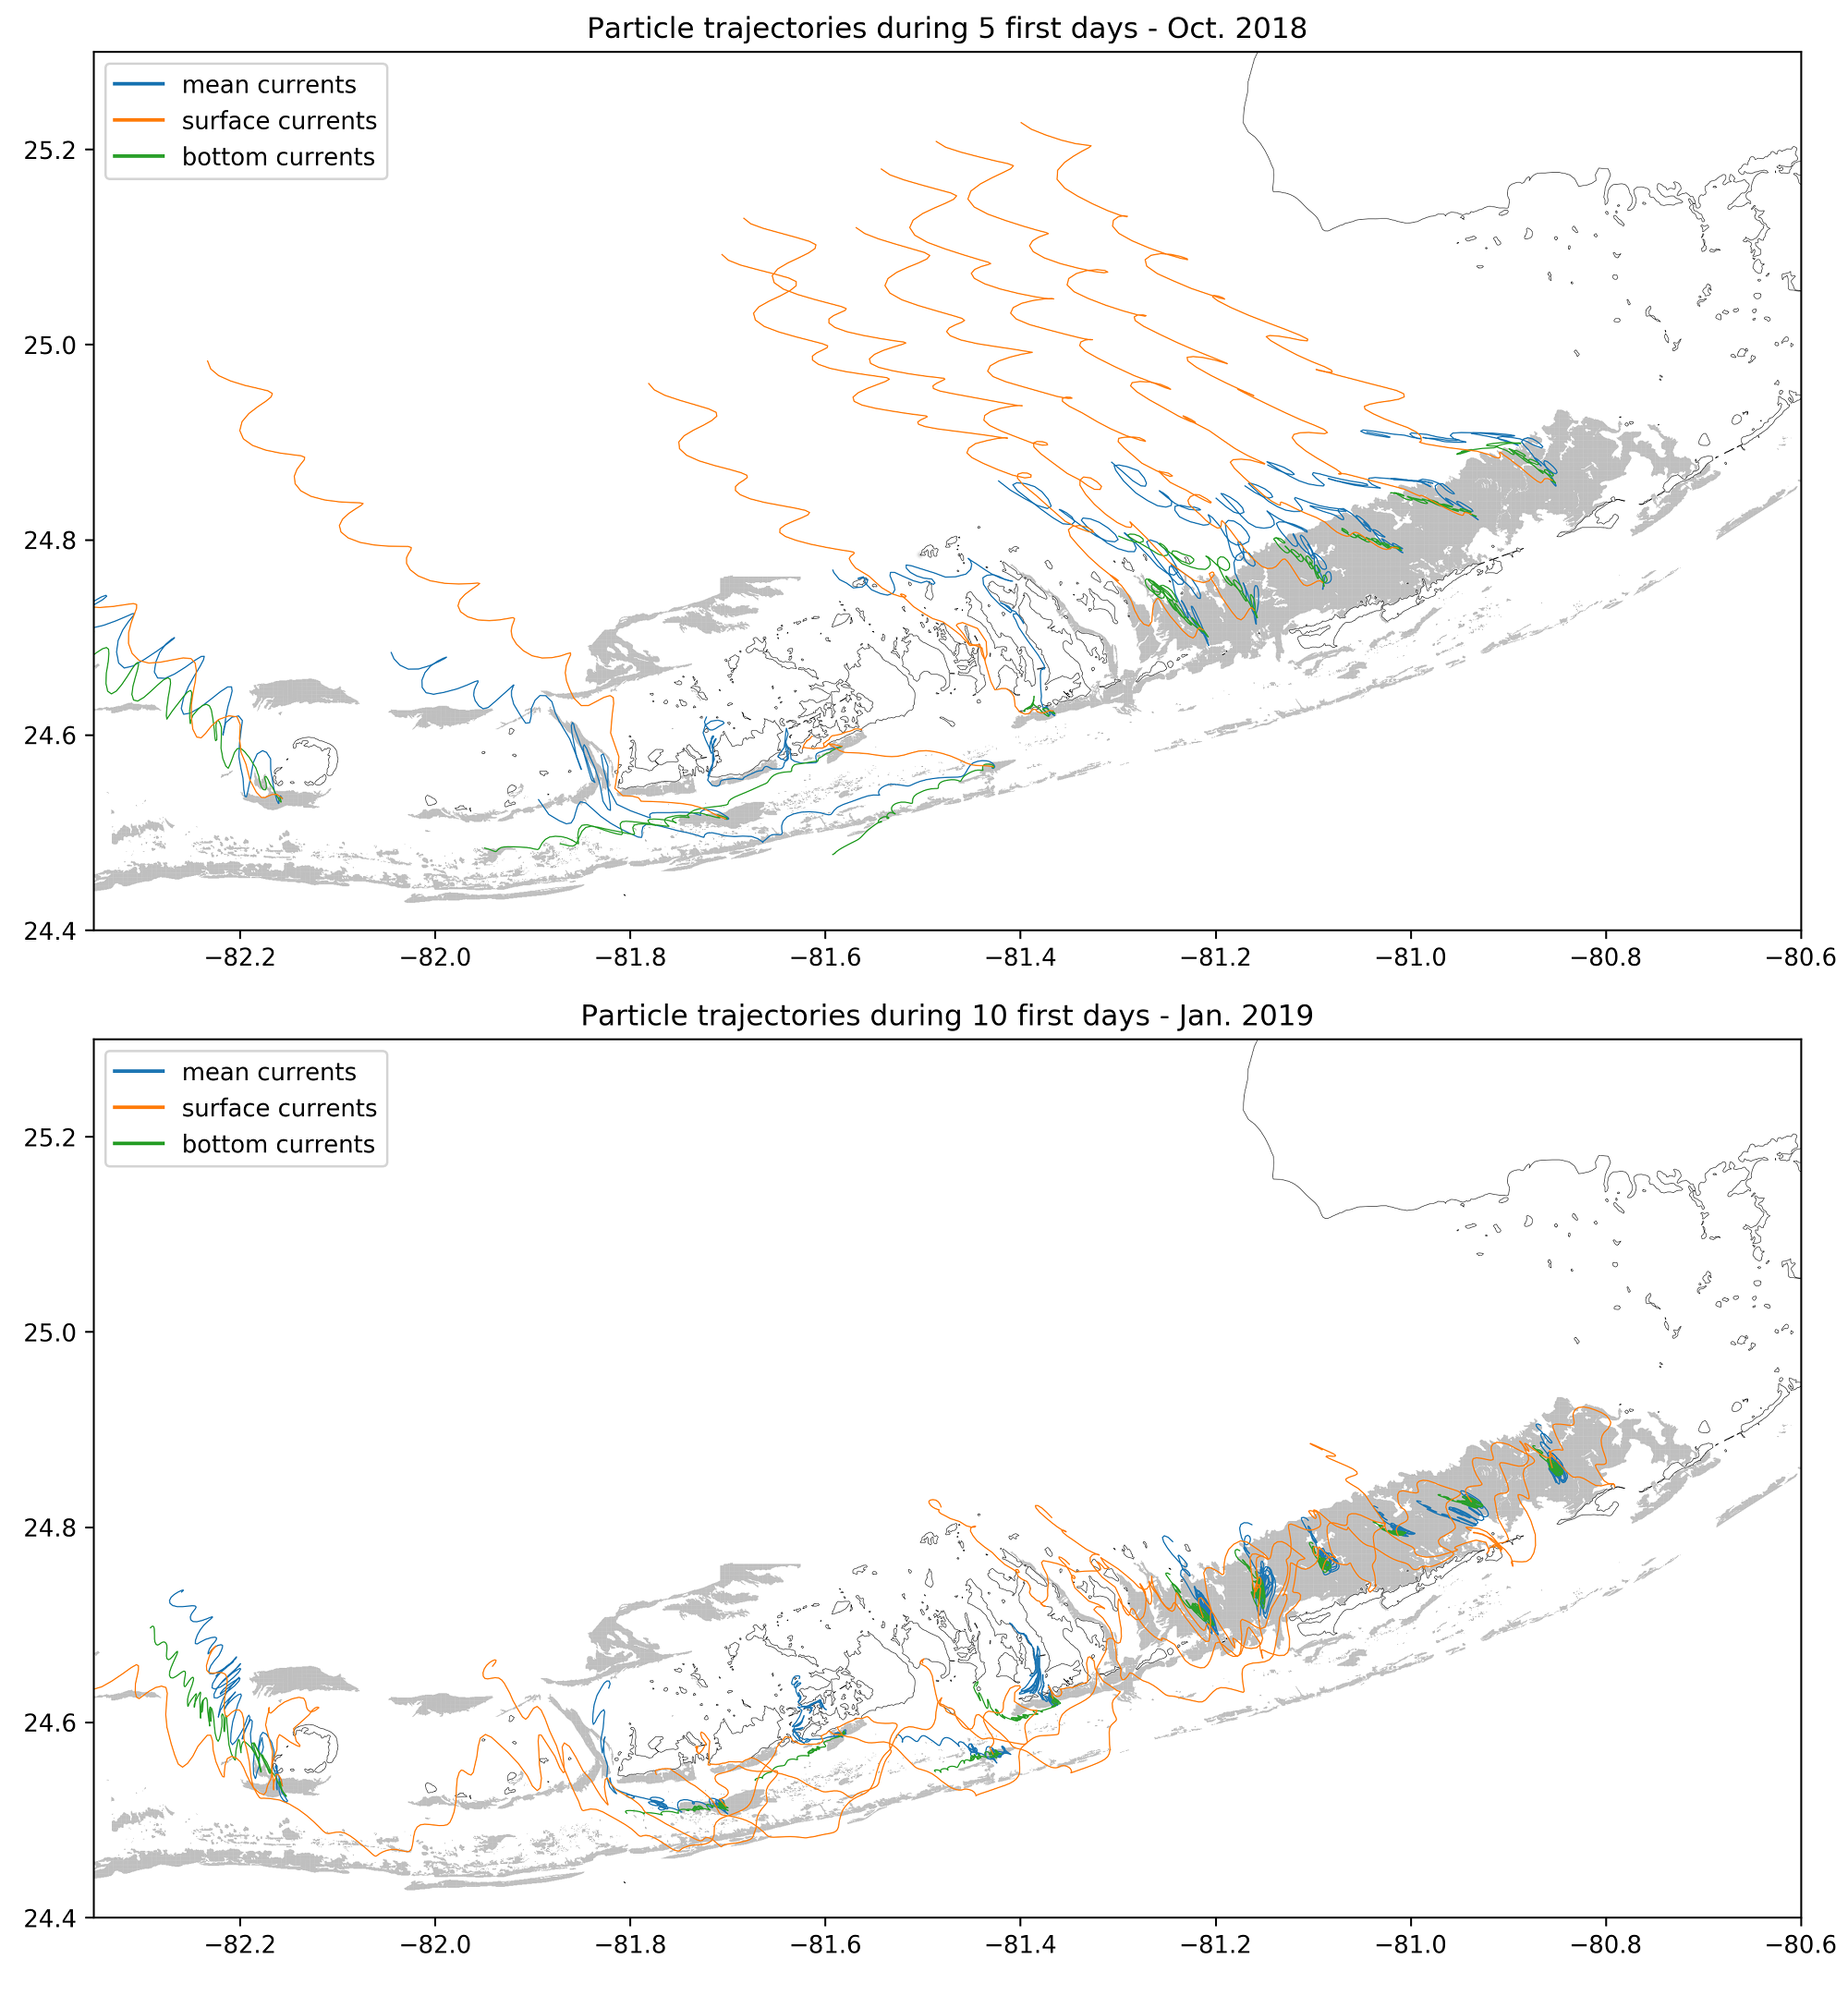
\includegraphics[width=.9\textwidth]{figures/traj.png}
    \caption{}
    \label{fig:traj}
\end{figure}

%\begin{figure}[h]
%    \centering
%    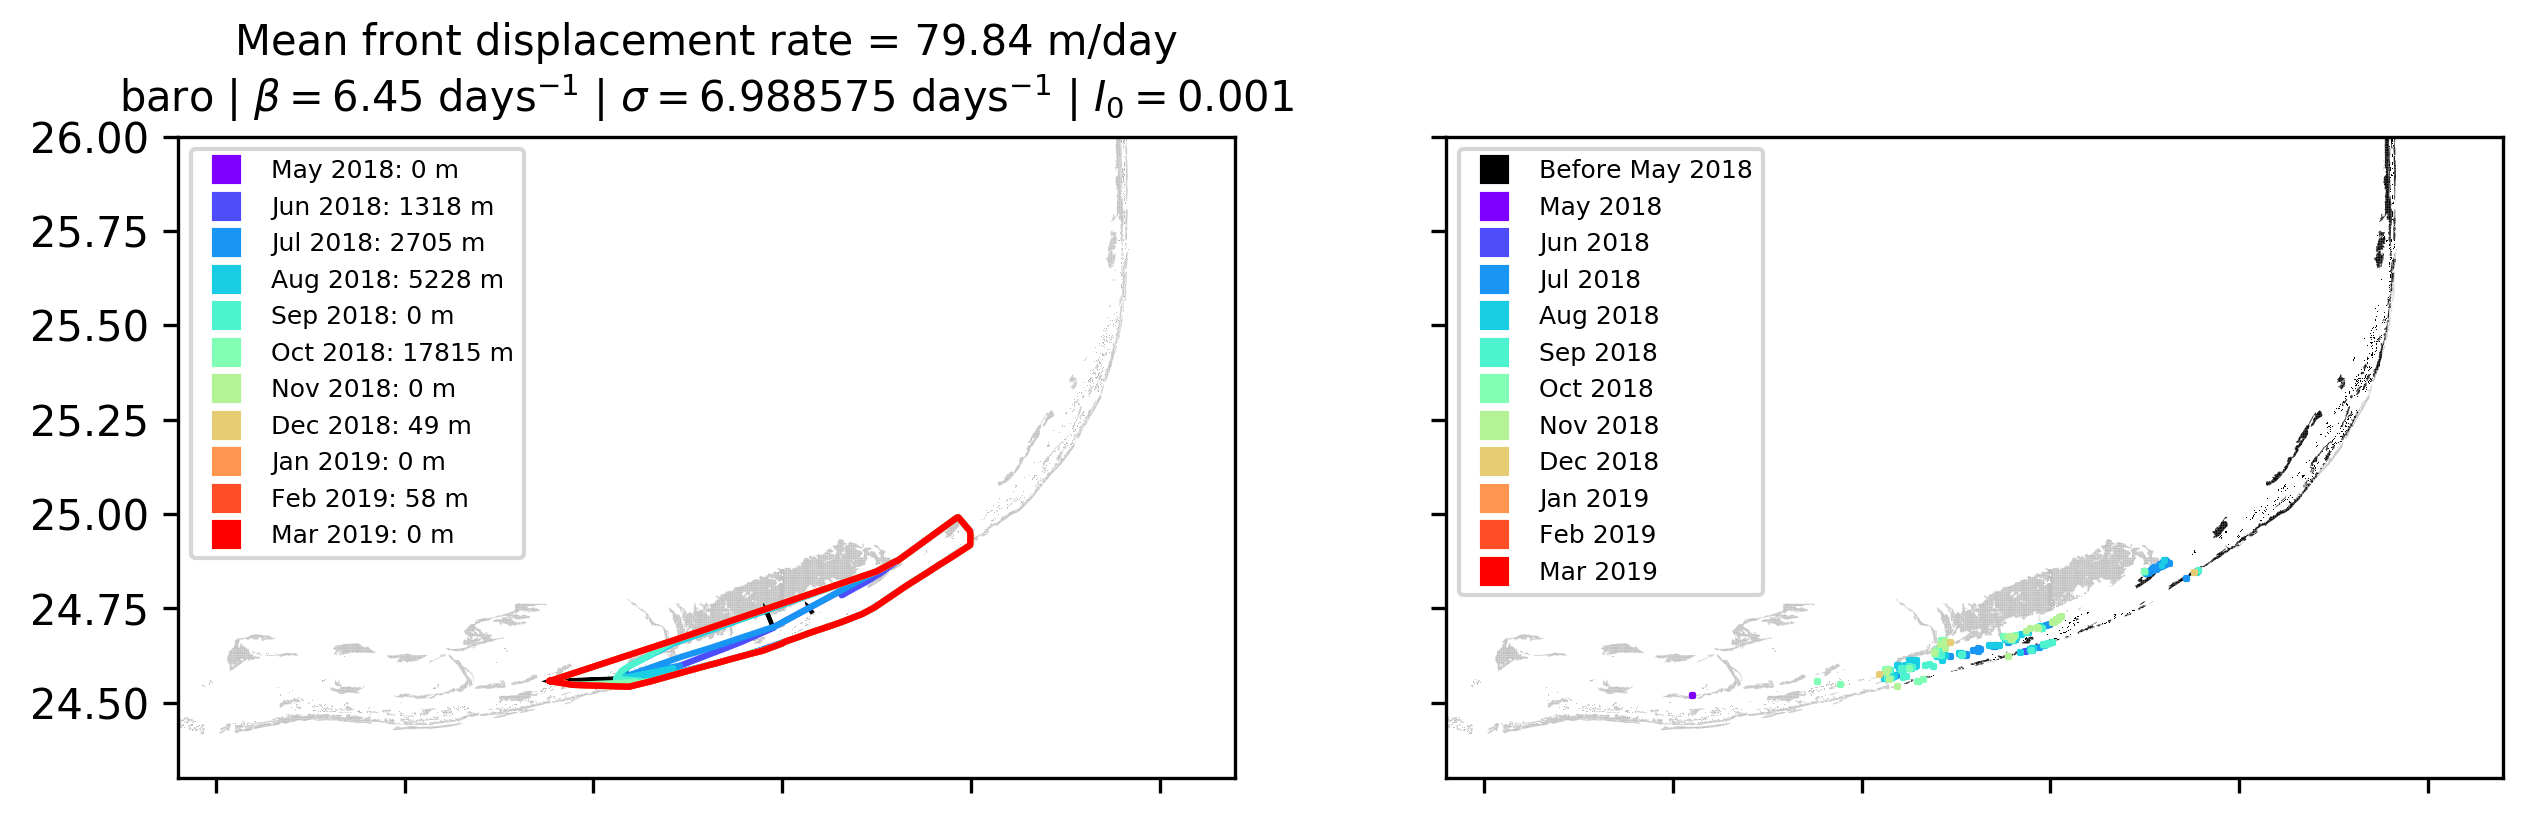
\includegraphics[width=.9\textwidth]{figures/hull_result.png}
%    \caption{Take home messages:\begin{itemize}
%        \item Our methods accurately captures disease front evolution through time (mtch between points and concave hulls)
%    \end{itemize}}
%    \label{fig:front}
%\end{figure}

% === DISCUSSION === %
\section{Discussion and conclusions}

\textcolor{blue}{Effect of waves and Stokes drift + 2D barotropic limitations ?}

In this model, the half life of the causative agent and its vector is proportional to the inverse of
particle mass depoition rate $\gamma$, ans is assumed to be 30 days. In the absence of data on $\gamma$, this seemed to be a reasonable assumption as particles life span would match the duration of the monthly simulations used to derive potential connectivity matrices \textcolor{blue}{(Any reference on degradation rate of organic matter in seawater ?)}. Nonetheless, the impact of $\gamma$ was assessed by performing Lagrangian tracking experiments of particles with a half life of 15 days. Increasing $\gamma$ strengthens short range connections while weakening short range connections. However, the decrease of long range connection probability remains limited as both values of $\gamma$ gave matrices with similar weighted connectivity lengths. Moreover, close to no variation was observed in reefs outdegrees. Therefore, although good calibration of $\gamma$ would give more accurate estimations of the probabilities of exchanges of infected materials over short distances, variation of this parameter should have minor impact on the conclusions of our simulations.

\textcolor{blue}{Discuss why same value for $\beta$ and $\beta_0'$ ?}

\textcolor{blue}{Discussion over method used to compute front speed ?}


Coral resistance to the SCTLD in modeled by parameter $I_0$, defined as the maximum proportion of the colony that can get infected without causing the disease to spread to the rest of the colony. Our simulations suggest that this value must be fairly low (around 0.01\%) in order for the disease to spread from reef to reef. This seems to imply that susceptible coral species have very weak defense mechanisms against the causative agent of the disease. \textcolor{blue}{What can we deduce from that, biologically speaking ?}

Furthermore, the appearance of an interval of optimal values of threshold $I_0$ for the propagation of the disease in our results highlights the impact of coral resistance on the spread of SCTLD through the FRT. On the one hand, when corals are strongly susceptible to the disease, infectious individuals are removed of the system too fast to become sustainable sources of infectious materials in the network. On the other hand, if corals are weakly susceptible to the disease, very few corals get infected and the disease barely propagates. Therefore, a further step in our modeling approach would be further dividing coral populations of our polygons into highly susceptible (\eg \textit{Dichocoenia stokesii}, \textit{Meandrina meandrites}), intermediately susceptible (\eg \textit{Orbicella faveolata}, \textit{Montastrea cavernosa}), and weakly susceptible (\eg \textit{Acropora Palmata}, \textit{Acropora cervicornis}) sub-populations. The proportions susceptible, infectious and removed individuals within these sub-populations would then be modeled with specific transmission ($\beta$, $\beta_0'$) and removal ($\sigma$) rates as well as specific infection thresholds $I_0$. Such approach would however require a fine knowledge of the distribution of the different coral species throughout the FRT. 

Another improvement of the model could be taking coral coverage into account. Currently, coral density is assumed homogeneous on the whole FRT. Consequently, coral population on a given reef becomes a function of its size, potentially causing the model to account for coral colonies where there are none. In areas such as Vaca reef, this leads the model to overestimate the spread of the SCTLD inside the reef. On other areas, however, as virtual particles are released on the whole reef area, propagation from reef to reef might also be overestimated. Nonetheless, these results can be improved by multiplying the rows and columns of the potential connectivity matrices corresponding to each polygon by the fraction of its area covered with coral. Again, refined data would be needed.

\textcolor{blue}{Should we say that our framework could be used in other locations touched by SCTLD, provided that data is available to deduce epidemiological parameters ?}

% potential critics/next steps

% === APPENDIX === %
%\appendix
\section*{Appendix}

% --- MODEL FORMULATION --- %
\subsection*{Subsection 1}
% --- MODEL EVALUATION --- %
\subsection*{Subsection 2}

\section*{Conflict of Interest Statement}
The authors declare that the research was conducted in the absence of any commercial or financial relationships that could be construed as a potential conflict of interest.

\section*{Author Contributions}
  
\section*{Funding}
This paper is a result of research funded by the Florida Department of Environmental Protection under award XXX to Mote Marine Laboratory. 

\section*{Acknowledgments}
Computational resources were provided by the Consortium des \'Equipements de Calcul Intensif (\textsc{c\'eci}), funded by the \textsc{f.r.s.-fnrs} under Grant No. 2.5020.11.

\section*{Supplemental Data}

% === BIBLIOGRAPHY === %
\bibliographystyle{frontiersinSCNS_ENG_HUMS} 
\bibliography{./biblio.bib}

%%% Make sure to upload the bib file along with the tex file and PDF
%%% Please see the test.bib file for some examples of references

\section*{Tables and figures}


\end{document}
